%                \begin{equation}\label{eq:Eq1}
%                    a+b = c
%                \end{equation}
%                \myequations{Une équation simple}
%                \begin{figure}[htp]
%                    \centering
%                    {\fbox{
\includegraphics[width = 0.8\textwidth]{figures/placeholder}}}
%                    \caption{Exemple de figure}
%                \end{figure}
%                \begin{lstlisting}[caption={Un code Python}]
%print("This line will be printéd.")
%print("Another line to print."\end{lstlisting}
%                \begin{tcolorbox}[colback=linkborder_Color!5!white,colframe=linkborder_Color!75!black]
%                    \textit{Ceci est un exemple d'encadré. Il sert à mettre en évidence des parties importantes du rapport}
%                \end{tcolorbox}
%                \begin{table}[H]
%                    \centering
%                    \begin{tabular}{lcccc}
%                        \toprule
%                        \textbf{Donnée} & \textbf{} & \textbf{} & \textbf{} & \textbf{} \\
%                        \midrule
%                         &  &  &  &  \\
%                         &  &  &  &  \\
%                         &  &  &  &  \\
%                         &  &  &  &  \\
%                        \bottomrule
%                    \end{tabular}
%                    \caption{Exemple de tableau}
%                \end{table}
%                \begin{table}[H]
%                    \centering
%                    \begin{tabular}{p{0.2\textwidth}|u|d|t|q} \toprule
%                        \textbf{Tâche} &  &  &  &
%                        \\
%                        \midrule
%                        \textbf{Donnée}&  &  & 0 & 0\\
%                        \bottomrule
%                    \end{tabular}
%                    \caption{Exemple de tableau coloré}
%                \end{table}
%
%            Let's mention this \cite{citation_key_online}
%
%            \begin{figure}[H]
%                \centering
%                    \subfloat[Sous-légende]{\fbox{
%                        
\includegraphics[width = 0.28\textwidth]{figures/placeholder}}}\qquad
%                    \subfloat[Sous-légende]{\fbox{
%                        
\includegraphics[width = 0.28\textwidth]{figures/placeholder}}}\qquad
%                    \subfloat[Sous-légende]{\fbox{
%                        
\includegraphics[width = 0.28\textwidth]{figures/placeholder}}}\qquad
%                    \subfloat[Sous-légende]{\fbox{
%                        
\includegraphics[width = 0.28\textwidth]{figures/placeholder}}}\qquad
%                    \subfloat[Sous-légende]{\fbox{
%                        
\includegraphics[width = 0.28\textwidth]{figures/placeholder}}}\qquad
%                    \subfloat[Sous-légende]{\fbox{
%                        
\includegraphics[width = 0.28\textwidth]{figures/placeholder}}}\qquad
%                    \subfloat[Sous-légende]{\fbox{
%                        
\includegraphics[width = 0.28\textwidth]{figures/placeholder}}}\qquad
%                    \subfloat[Sous-légende]{\fbox{
%                        
\includegraphics[width = 0.28\textwidth]{figures/placeholder}}}\qquad
%                    \subfloat[Sous-légende]{\fbox{
%                        
\includegraphics[width = 0.28\textwidth]{figures/placeholder}}}\qquad
%                \caption{Exemple avec plusieurs figures}
%
%            \end{figure}


\chapter{Direction des énergies et Centre de Grenoble}\label{ch:direction-des-energies-et-centre-de-grenoble}


\section{Origines et contributions à la recherche sur les énergies}\label{sec:origines-et-contributions-a-la-recherche-sur-les-energies}

Comme de nombreuses autres entités industrielles et universitaires (Groupe EDF, Groupe INSA \ldots), le Commissariat à l'Énergie Atomique
tire ses origines des suites de la Seconde Guerre Mondiale et du besoin de réindustrialisation en France et en Europe à cette période.
En particulier, le largage des bombes atomiques américaines sur Hiroshima et Nagasaki en août 1945 motive le gouvernement provisoire, présidé par Charles de Gaulle, à mettre en place un organisme de recherche pour l'énergie atomique : c'est la naissance du \gls{CEA}, avec à sa tête Frédéric Joliot-Curie \textit{(jusqu'alors directeur du CNRS, gendre de Pierre et Marie Curie et Prix Nobel de chimie)} comme haut-commissaire à l'énergie atomique et Raoul Dautry comme administrateur général.

    Les activités de recherche de l'organisme se concentrent dans un premier temps sur l'énergie nucléaire \textit{(création du centre d'études nucléaires de Saclay en 1952, création de réacteurs militaires à Marcoule à la fin des années 50, collaboration avec EDF pour la construction des premiers réacteurs civils à Chinon dans les années 60)}\cite{wiki_CEA}

    Ses domaines d'expertise se diversifient progressivement avec notamment une activité européenne en calcul intensif \textit{(création d'un laboratoire spécialisé dans les supercalculateurs en collaboration avec le CNRS et Intel)}, en recherche fondamentale, en microélectronique, en défense, en biologie et en technologies pour la santé.

    Ainsi, le \gls{CEA} se place désormais comme une structure de premier plan sur les scènes nationale et internationale en matière de recherche technologique.
    Ses activités de recherche sont structurées autour de quatre Directions Opérationnelles (figure~\ref{fig:organigramme-CEA}), principalement implantées sur 8 centres (figure~\ref{fig:organigramme-Centres}) et assistées par les directions fonctionnelles \textit{(direction financière, direction juridique, direction des systèmes d'information, direction des relations internationales, direction de la communication...)}

    Sur le plan juridique, il fait partie des \gls{odac} et des \gls{epic}.
    Il est dirigé par une administratrice générale\footnote{très récemment nommée par le Président de la République \textit{(juillet 2025)}} assisté par son adjoint\footnote{dont la nomination est encore plus récente \textit{(quelques semaines à date d'écriture du rapport)} et jusqu'alors directeur du Centre de Grenoble}

    Les travaux du \gls{CEA} valent à ses auteurs plusieurs distinctions très prestigieuses :
    \begin{itemize}
        \item Première place au classement Reuters des organismes en termes d'innovation en 2016
        \item Prix Nobel de physique à Anne L'Huillier\footnote{envers qui l'INSA CVL est redevable d'une passionnante conférence sur l'échelle attoseconde le 4 décembre dernier} et Pierre Agostini en 2023, et Michel Devoret en 2025, respectivement pour leurs travaux sur les impulsions lasers attoseconde et les circuits électroniques quantiques
    \end{itemize}

    \begin{figure}[H]
        \centering
        % Le contenu du diagramme est défini dans le fichier suivant
        \fbox{\begin{tikzpicture}[
    main/.style={text centered, text width=10cm, fill=red!20, draw, rectangle, rounded corners, font=\bfseries\Large},
    direction/.style={text centered, text width=3cm, fill=gray!50, draw, rectangle, rounded corners},
    institut/.style={grow=down, xshift=4cm, text centered, text width=5cm, draw, rectangle, rounded corners, edge from parent path={(\tikzparentnode.225) |- (\tikzchildnode.west)}},
    first/.style    ={level distance=15ex},
    second/.style   ={level distance=30ex},
    third/.style    ={level distance=45ex},
    fourth/.style   ={level distance=60ex},
    fifth/.style    ={level distance=75ex},
    level 1/.style={sibling distance=12.5em, level distance=8em}]

    \node[main, anchor=south]{Direction Générale du CEA}
    [edge from parent fork down]
    %
    child{node (d1) [direction] {\textbf Direction \\ des \textbf Énergies}
    child[institut,first] {node {\textbf{I}nstitut de {R}echerche\\ et d'{É}{\textbf t}ude{\textbf s} en {É}conomie\\ de l'\textbf{É}nergie}}
    child[institut,second] {node {\textbf{L}aboratoire d'\textbf{I}nnovation\\ pour les \textbf{T}echnologies des\\ \textbf{É}nergies {N}ouvelles et\\ les \textbf{N}anomatériaux}}
    child[institut,third] {node {\textbf{I}nstitut des \textbf{S}ciences\\ \textbf{et} {T}echnologies pour une\\ \textbf{É}conomie \textbf{C}irculaire\\ des {é}nergies bas carbone}}
    child[institut,fourth] {node {\textbf{I}nstitut de \textbf{Re}cherche\\ pour les \textbf{S}ystèmes \textbf{N}ucléaires\\ pour la production d'\textbf{É}nergie bas carbone}}
    child[institut,fifth] {node {\textbf{I}nstitut des \textbf{S}ciences\\ \textbf{A}ppliquées et de la \textbf{S}imulation\\ pour les {É}nergies carbone}}
    }
    %
    child{node (d2) [direction] {\textbf Direction \\ des \textbf{A}pplications \textbf{M}ilitaires}}
    %
    child{node (d3) [direction] {\textbf Direction \\ de la \textbf{R}echerche \textbf{T}echnologique}}
    %
    child{node (d4) [direction] {\textbf Direction \\ de la \textbf{ R}echerche \textbf{F}ondamentale}};

\end{tikzpicture}}
        \caption{Organigramme simplifié des Directions Opérationnelles du CEA}
        \label{fig:organigramme-CEA}
    \end{figure}

    \begin{figure}[H]
        \centering
        % Le contenu du diagramme est défini dans le fichier suivant
        \fbox{\begin{tikzpicture}[
    main/.style={text centered, text width=10cm, fill=red!50, draw, rectangle, rounded corners, font=\bfseries\Large},
    direction/.style={text centered, text width=3cm, fill=orange!20, draw, rectangle, rounded corners, font=\large},
    institut/.style={grow=down, xshift=3cm, text centered, text width=4cm, draw, rectangle, rounded corners, edge from parent path={(\tikzparentnode.225) |- (\tikzchildnode.west)}},
    site/.style={level distance = 6ex, xshift=4.5cm, text centered, text width=5cm, draw, rectangle, rounded corners, edge from parent path={(\tikzparentnode.225) |- (\tikzchildnode.west)}},
    first/.style    ={level distance=12ex},
    second/.style   ={level distance=24ex},
    third/.style    ={level distance=36ex},
    fourth/.style   ={level distance=48ex},
    fifth/.style    ={level distance=60ex},
    level 1/.style={sibling distance=30em, level distance=5em}]

    \node[main, anchor=south]{Direction Générale du CEA}
    [edge from parent fork down]
    %
    child{node (d1) [direction] {Centres civils}
        child[institut,first]  {node {Centre de Cadarache}}
        child[institut,second] {node {Centre de Grenoble}
            child[site]  {node {\textbf Institut \textbf National de l'\textbf Énergie \textbf Solaire (Chambéry)}}
        }
        child[institut,third]  {node {Centre de Marcoule}}
        child[institut,fourth] {node {Centre de Paris-Saclay}}
    }
    %
    child{node (d2) [direction] {Centres Militaires}
        child[institut,first]  {node {Centre du Cesta}}
        child[institut,second] {node {Centre de Gramat}}
        child[institut,third]  {node {Centre du Ripault}}
        child[institut,fourth] {node {Centre de Valduc}}
        child[institut,fifth] {node {Centre DAM Île-de-France}}
    };
\end{tikzpicture}}
        \caption{Organigramme simplifié des Centres du CEA}
        \label{fig:organigramme-Centres}
    \end{figure}

Citons enfin quelques chiffres-clés du \gls{CEA}\cite{CEA_prez_generale}, publiés à l'occasion des 80 ans de l'organisme, pour conclure cette introduction.
    \begin{itemize}
        \item 6,4 milliards d'euros de budget militaire et civil
        \item 22 105 salariés, dont 1154 alternants et 1469 doctorants, avec un ratio Hommes/Femmes de 13 pour 7
        \item 4757 publications scientifiques dont 65\% de publications internationales
        \item 1er déposant de brevets en France et en Europe
        \item 405 projets européens acceptés
        \item 260 start-up créées depuis 1972, dont 80\% en activité après 10 ans et 13 nouvelles en 2024
        \item 700 partenaires industriels dont 42\% de PME
    \end{itemize}

    \begin{tcolorbox}[colback=linkborderColor!5!white,colframe=linkborderColor!75!black]
        Il est intéressant de s'attarder sur ces chiffres et ce qu'ils révèlent sur la stratégie du \gls{CEA}.

        En effet, il est peu commun qu'une entreprise compte une telle proportion de doctorants et d'alternants dans ses rangs.
        Ceci illustre la volonté du \gls{CEA} d'inscrire son développement sur un temps long en attirant des profils jeunes et en leur offrant une formation de haut niveau dans un environnement technologique de pointe, les Centres du \gls{CEA} étant tous composés de bureaux mais également d'équipements de recherche innovants.

        Le modèle économique du \gls{CEA} est par ailleurs particulier en ce que celui-ci relève d'une part du Service Public par son intrication avec le gouvernement \textit{(administration générale nommée par le Président de la République)} et d'autre part du monde industriel privé investi par ses collaborateurs, lesquels sont pour la plupart des entreprises de différentes tailles.
        Ainsi, le bon fonctionnement de l'organisme est contraint par le financement de ses brevets par les partenaires industriels, abondé par des subventions publiques.
        Cette contrainte est double car elle impose au \gls{CEA} de conserver une crédibilité scientifique et commerciale devant l'ensemble des acteurs de la recherche technologique.
        Son image de marque est donc importante.
    \end{tcolorbox}

    \newpage\subsection{Direction des énergies}\label{subsec:direction-des-energies}

Le dernier rapport d'activités~\cite{CEA_prez_DES} de la \gls{DES} structure son activité selon 5 axes :
        \begin{enumerate}
            \item Produire des énergies bas carbone
            \item Stocker les énergies et développer les nouveaux vecteurs
            \item Optimiser les ressources
            \item Concevoir et gérer les installations
            \item Accompagner et valoriser les activités
        \end{enumerate}

        Plus concrètement, les avancées du \gls{CEA} en matière d'énergie concernent l'ensemble du mix bas-carbone :
        \begin{itemize}
            \item Le nucléaire de 3ème génération \textit{(Calculs CFD sur de très gros volumes de données, création d'un jumeau numérique d'un réacteur nucléaire, amélioration continue des équipements de sûreté \ldots)}
            \item Le nucléaire par \gls{SMR}, notamment avec de potentielles applications en production de chaleur industrielle et d'hydrogène bas-carbone
            \item Le solaire avec le développement du photovoltaïque et notamment du photovoltaïque spatial \textit{(panneaux solaires plus légers et moins volumineux destinés à être embarqués dans les lanceurs spatiaux)} et les cellules à hétérojonction \textit{(utilisation de deux matériaux semi-conducteurs différents)} pour lesquelles un record de rendement \textit{(25\%)} a été atteint
            \item Les batteries électriques avec des travaux sur l'hybridation ainsi que sur l'emballement thermique
            \item L'hydrogène, avec des activités sur le stockage \textit{(matériaux biosourcés)} et sur la production \textit{(méthode de production décarbonée par énergie solaire)}
            \item Les carburants durables \textit{(biocarburants, catalysation du $\textrm {CO}_2$)}
            \item L'efficacité et la sobriété \textit{(optimisation des réseaux de chaleur urbains, production de froid)}
            \item L'analyse approfondie des cycles de vie des systèmes énergétiques
        \end{itemize}

    \begin{tcolorbox}[colback=linkborderColor!5!white,colframe=linkborderColor!75!black]
        Ces éléments illustrent la volonté du \gls{CEA} d'impacter l'ensemble des domaines de recherche technologique, révélant une stratégie intéressante dans un contexte mondial de forte tension à plusieurs niveaux, notamment sur l'accès aux ressources et aux chaînes d'approvisionnement.
        C'est en ce sens qu'une étude a été menée conjointement par le \gls{CEA} et le Ministère de la Transition Écologique en 2023 pour évaluer l'évolution de l'offre et de la demande mondiales de lithium après 2050, montrant à nouveau des objectifs affichés de planification à long terme des activités de l'organisme.
    \end{tcolorbox}

% Focus sur Grenoble + histoire
\newpage\section{Le Centre CEA de Grenoble : entre diversité des domaines de recherche et résilience historique}\label{sec:le-centre-cea-de-grenoble-:-entre-diversite-des-domaines-de-recherche-et-resilience-historique}

Le Centre de Grenoble et ses 4500 chercheurs forment le plus grand site du \gls{CEA} après celui de Paris-Saclay \textit{(7000 salariés)}\cite{CEA_Gre}.

Le Centre est fondé en 1956 par Louis Néel, prix Nobel de physique\cite{wiki_CEA_Grenoble}.
A l'origine destiné à la recherche nucléaire, le site connaît une transformation en profondeur à la suite du démantèlement de l'ensemble des installations nucléaires dans les années 2000, notamment ses trois célèbres réacteurs Mélusine, Siloé et Siloette.
Désormais, la recherche du Centre porte sur les nouvelles technologies de l'énergie, de la santé, de l'information et de la communication.
Ses activités sont principalement conduites par le \gls{LITEN}\footnote{Il convient de préciser que l'alternance rapportée ne se situe pas réellement à Grenoble mais sur le site de l'INES en Savoie, rattaché administrativement au Centre de Grenoble. Ainsi, l'INES fait partie des nombreuses autres antennes réparties sur tout le territoire français permettant de faire du CEA un acteur national de premier plan en matière de recherche technologique.}
et le \gls{LETI}, ce dernier étant responsable d'une partie importante du développement du Centre entre les années 70 et 2000 : on peut citer en particulier la start-up Efcis fondée en 1972 ayant donné naissance au groupe ST Microelectronics en 1992, comme exemple du positionnement privilégié du Centre dans l'écosystème technologique grenoblois et national.
Enfin, le \gls{CEA} Grenoble connaît une activité importante en recherche fondamentale portée par plus de mille collaborateurs.

\begin{tcolorbox}[colback=linkborderColor!5!white,colframe=linkborderColor!75!black]
    Ainsi, le Centre de Grenoble s'inscrit dans la politique générale du \gls{CEA} de garder un rôle de leader dans l'ensemble des domaines de la recherche technologique.
    On peut mentionner quelques chiffres éloquents sur l'ouverture du Centre à l'ensemble de son environnement\cite{CEA_Gre} : 500 partenaires industriels, des actions dans les établissements scolaires ayant touché plus de 3500 collégiens et lycéens, 38000 visiteurs sur les quelque 400 évènements scientifiques annuels organisés à la Maison Minatec à Grenoble.

    La résilience du Centre et sa capacité à résister à des difficultés majeures a été une nouvelle fois montrée en 2015 lors de l'incendie des salles blanches du \gls{LETI}, une zone de recherche remarquable du site, n'ayant pas empêché le \gls{CEA} de poursuivre son activité en microélectronique sans impact déterminant sur son image de marque.
\end{tcolorbox}

\begin{figure}[H]
    \centering
    % Le contenu du diagramme est défini dans le fichier suivant
    \fbox{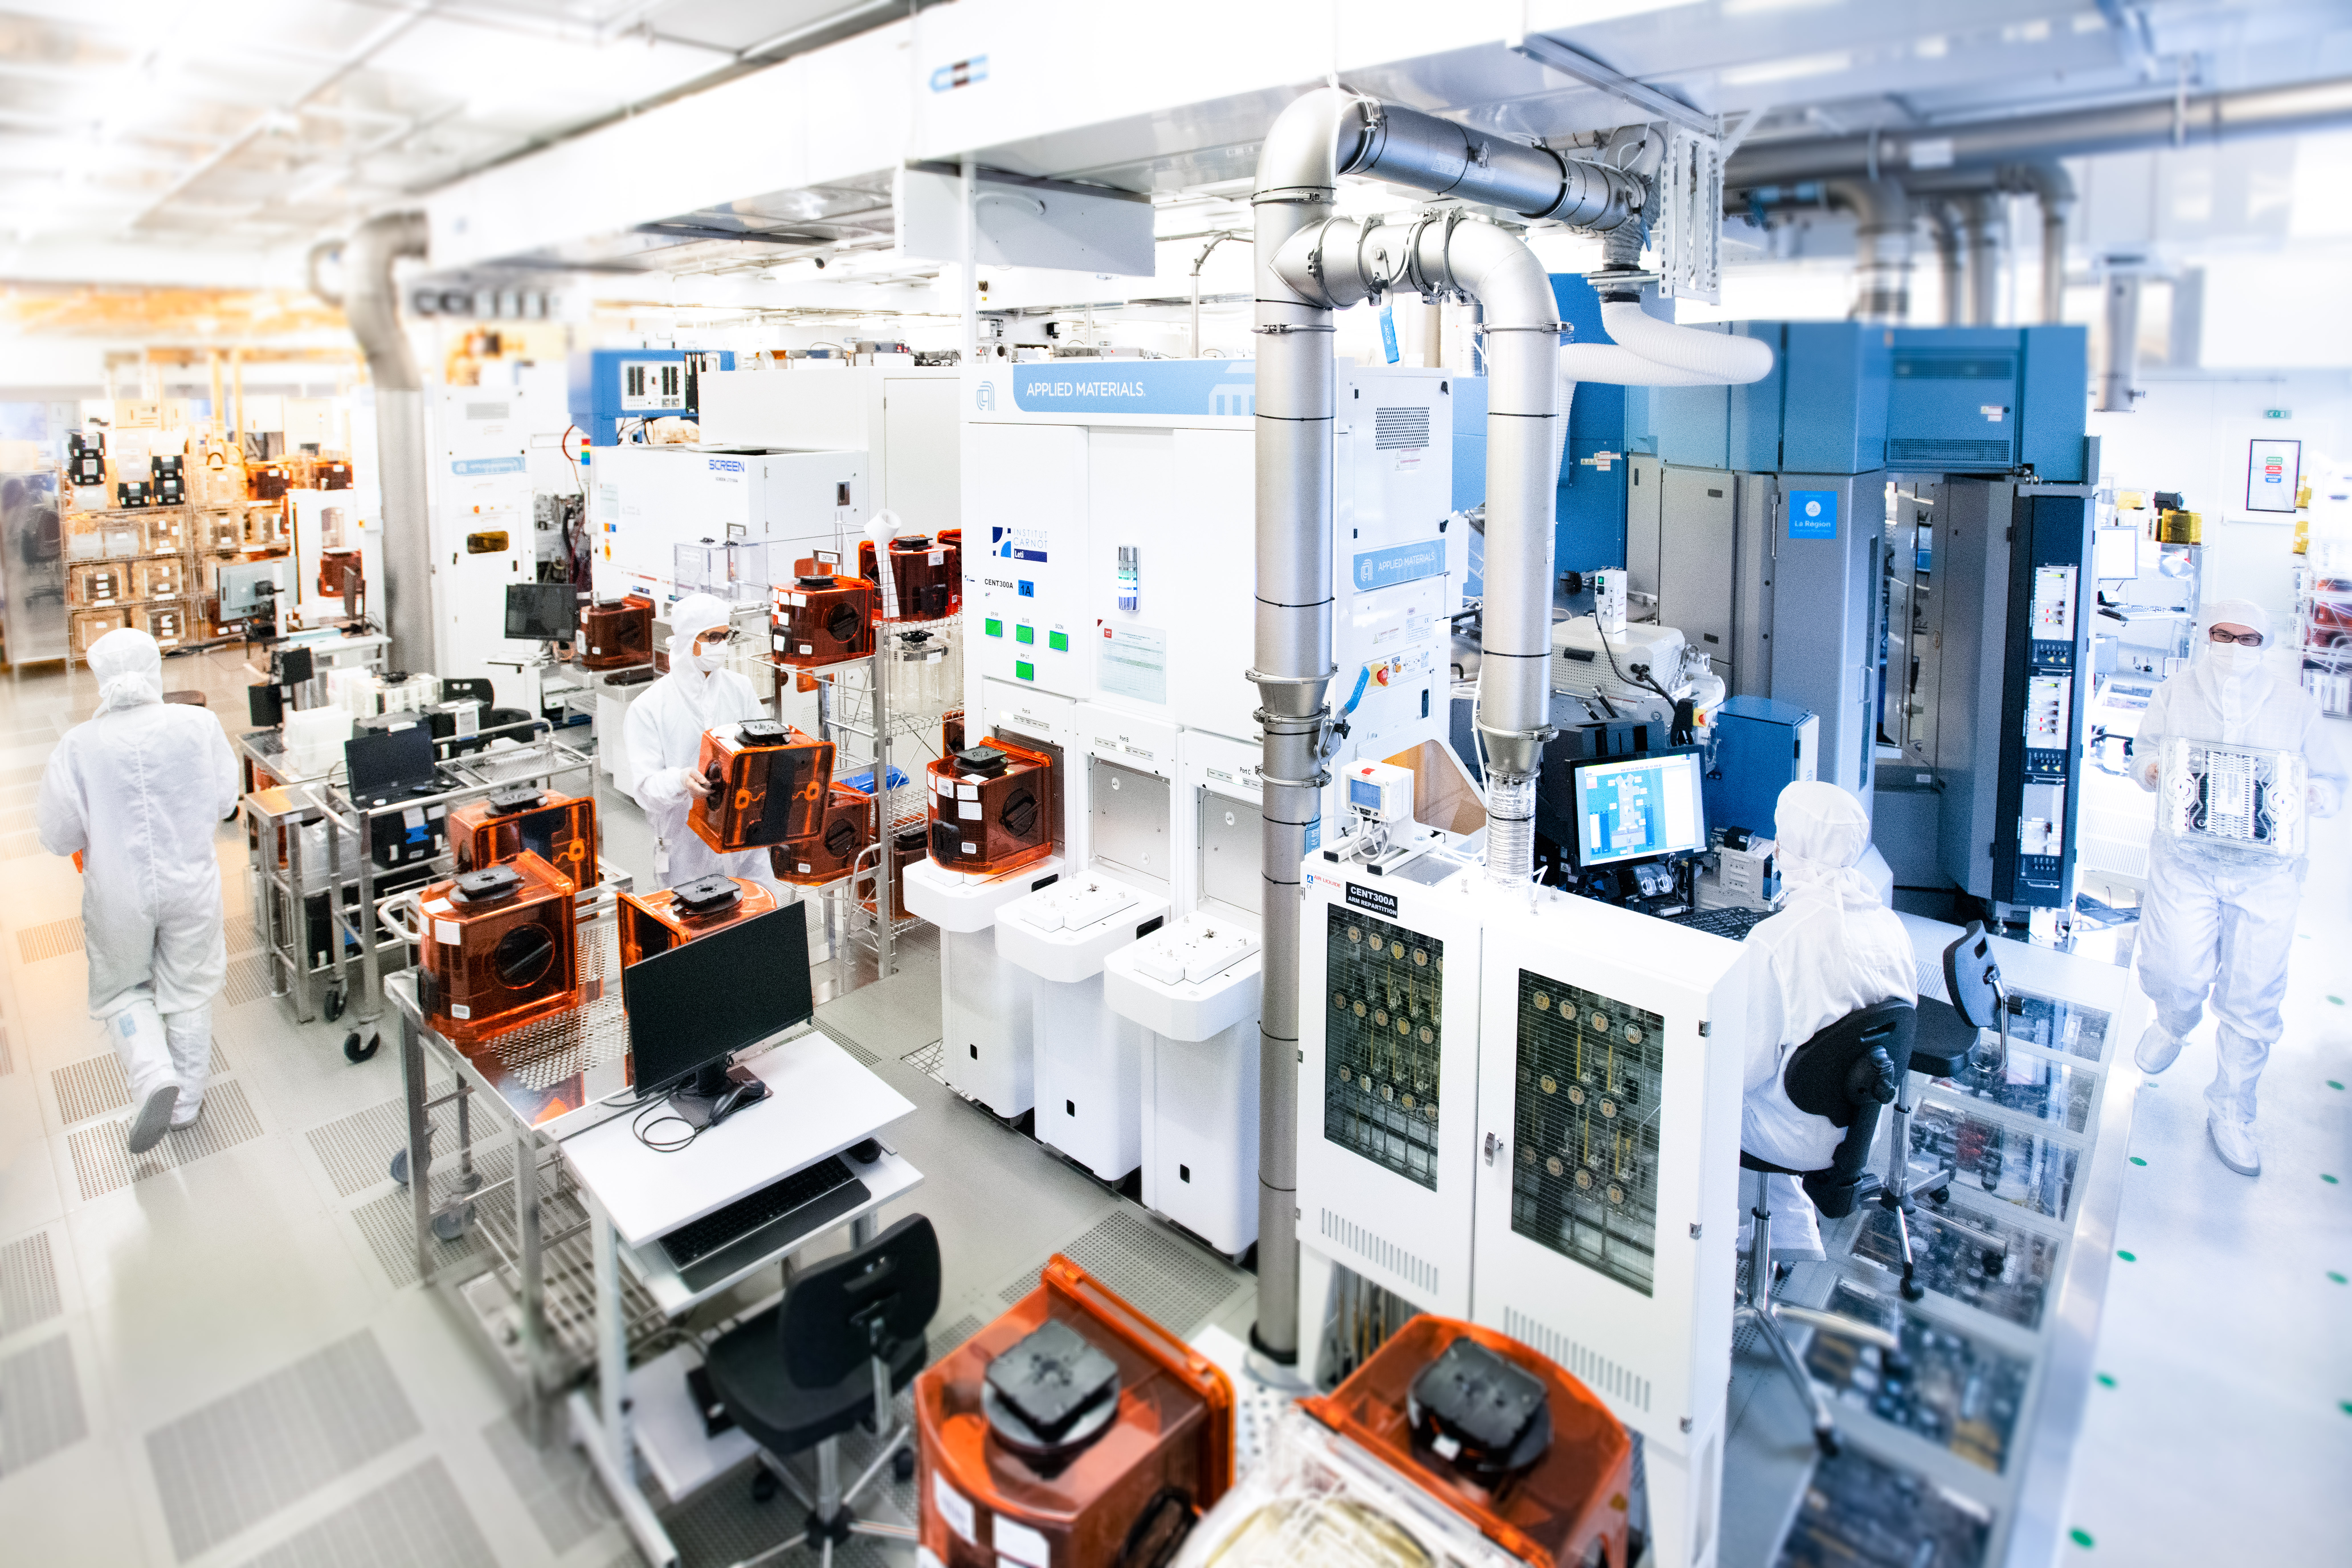
\includegraphics[width=0.9\textwidth]{figures/illustrations/photos/SB_A_AUBERT}}
    \caption{Une des salles blanches du LETI au CEA de Grenoble}
    \label{fig:SB}
\end{figure}


